\section{Problem 5}

\subsection{Code}


\begin{lstlisting}
function [IVec,QVec] = if2iq(xVec,T,fIF)
% IF2IQ : Convert intermediate frequency samples to baseband I and Q samples.
%
% Let x(n) = I(n*T)*cos(2*pi*fIF*n*T) - Q(n*T)*sin(2*pi*fIF*n*T) be a
% discrete-time bandpass signal centered at the user-specified intermediate
% frequency fIF, where T is the bandpass sampling interval. Then this
% function converts the bandpass samples to quadrature samples from a complex
% discrete-time baseband representation of the form xl(m*Tl) = I(m*Tl) +
% j*Q(m*Tl), where Tl = 2*T.
%
%
% INPUTS
%
% xVec -------- N-by-1 vector of intermediate frequency samples with
%               sampling interval T.
%
% T ----------- Sampling interval of intermediate frequency samples, in
%               seconds.
%
% fIF --------- Intermediate frequency of the bandpass signal, in Hz.
%
%
% OUTPUTS
%
% IVec -------- N/2-by-1 vector of in-phase baseband samples.
%
% QVec -------- N/2-by-1 vector of quadrature baseband samples.
%
%
%+------------------------------------------------------------------------------+
% References:
%
%
%+==============================================================================+
n = 0:1:length(xVec)-1; n=n';
IVec = 2*cos(2*pi*fIF*n*T).*xVec;
QVec = -2*sin(2*pi*fIF*n*T).*xVec; % figure out the sign

IVec = decimate(IVec,2)/sqrt(2);
QVec = decimate(QVec,2)/sqrt(2);
\end{lstlisting}


\begin{lstlisting}
function [xVec] = iq2if(IVec,QVec,Tl,fIF)
% IQ2IF : Convert baseband I and Q samples to intermediate frequency samples.
%
% Let xl(m*Tl) = I(m*Tl) + j*Q(m*Tl) be a discrete-time baseband
% representation of a bandpass signal. This function converts xl(n) to a
% discrete-time bandpass signal x(n) = I(n*T)*cos(2*pi*fIF*n*T) -
% Q(n*T)*sin(2*pi*fIF*n*T) centered at the user-specified intermediate
% frequency fIF, where T = Tl/2.
%
%
% INPUTS
%
% IVec -------- N-by-1 vector of in-phase baseband samples.
%
% QVec -------- N-by-1 vector of quadrature baseband samples.
%
% Tl ---------- Sampling interval of baseband samples (complex sampling
%               interval), in seconds.
%
% fIF --------- Intermediate frequency to which the baseband samples will
%               be up-converted, in Hz.
%
%
% OUTPUTS
%
% xVec -------- 2*N-by-1 vector of intermediate frequency samples with
%               sampling interval T = Tl/2.
%
%
%+------------------------------------------------------------------------------+
% References:
%
%
%+==============================================================================+
IVec_resampled = interp(IVec,2);
QVec_resampled = interp(QVec,2);

T = Tl/2;
n = 0:1:length(IVec_resampled)-1; n=n';
xVec = IVec_resampled.*cos(2*pi*fIF*n*T) ...
        - QVec_resampled.*sin(2*pi*fIF*n*T);

xVec = sqrt(2)*xVec;
\end{lstlisting}

\subsection{Results}

The power spectral density of the original signal (baseband representation),
the bandpass representation and the reconstructed baseband representation can
be observed in Figures~\ref{fig:ex5_baseband_original}, \ref{fig:ex5_bandpass}
and \ref{fig:ex5_baseband_reconstructed}, respectively. Note that the bandpass
representation had to be centered at a $f_{IF} = 5MHz$ to be able to reconstruct
the signal without distortion since the bandwidth of the original signal is
approximately 5MHz.

\begin{figure}[H]
	\centering
	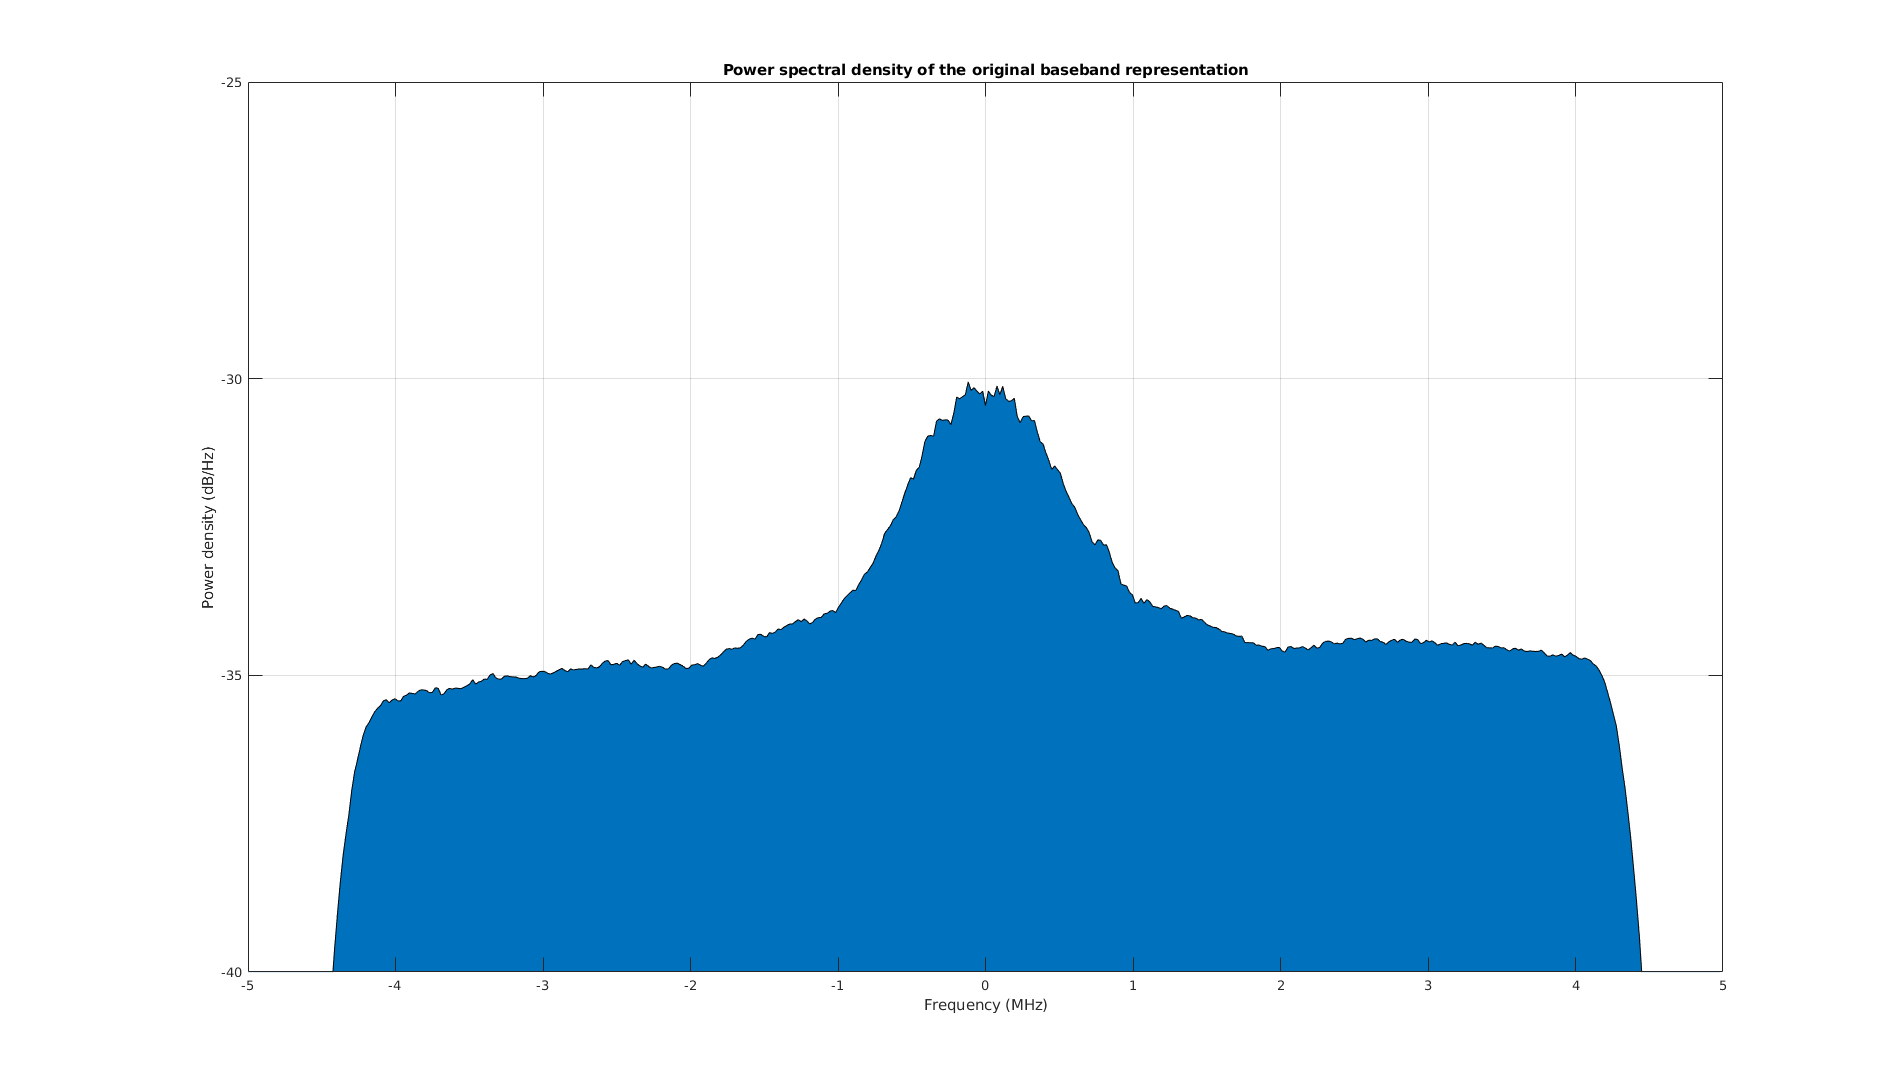
\includegraphics[width=0.9\textwidth]{figs/PSD_baseband_original.png}
	\caption{Power spectral density of the original signal in its baseband
		representation.}
	\label{fig:ex5_baseband_original}
\end{figure}

\begin{figure}[H]
	\centering
	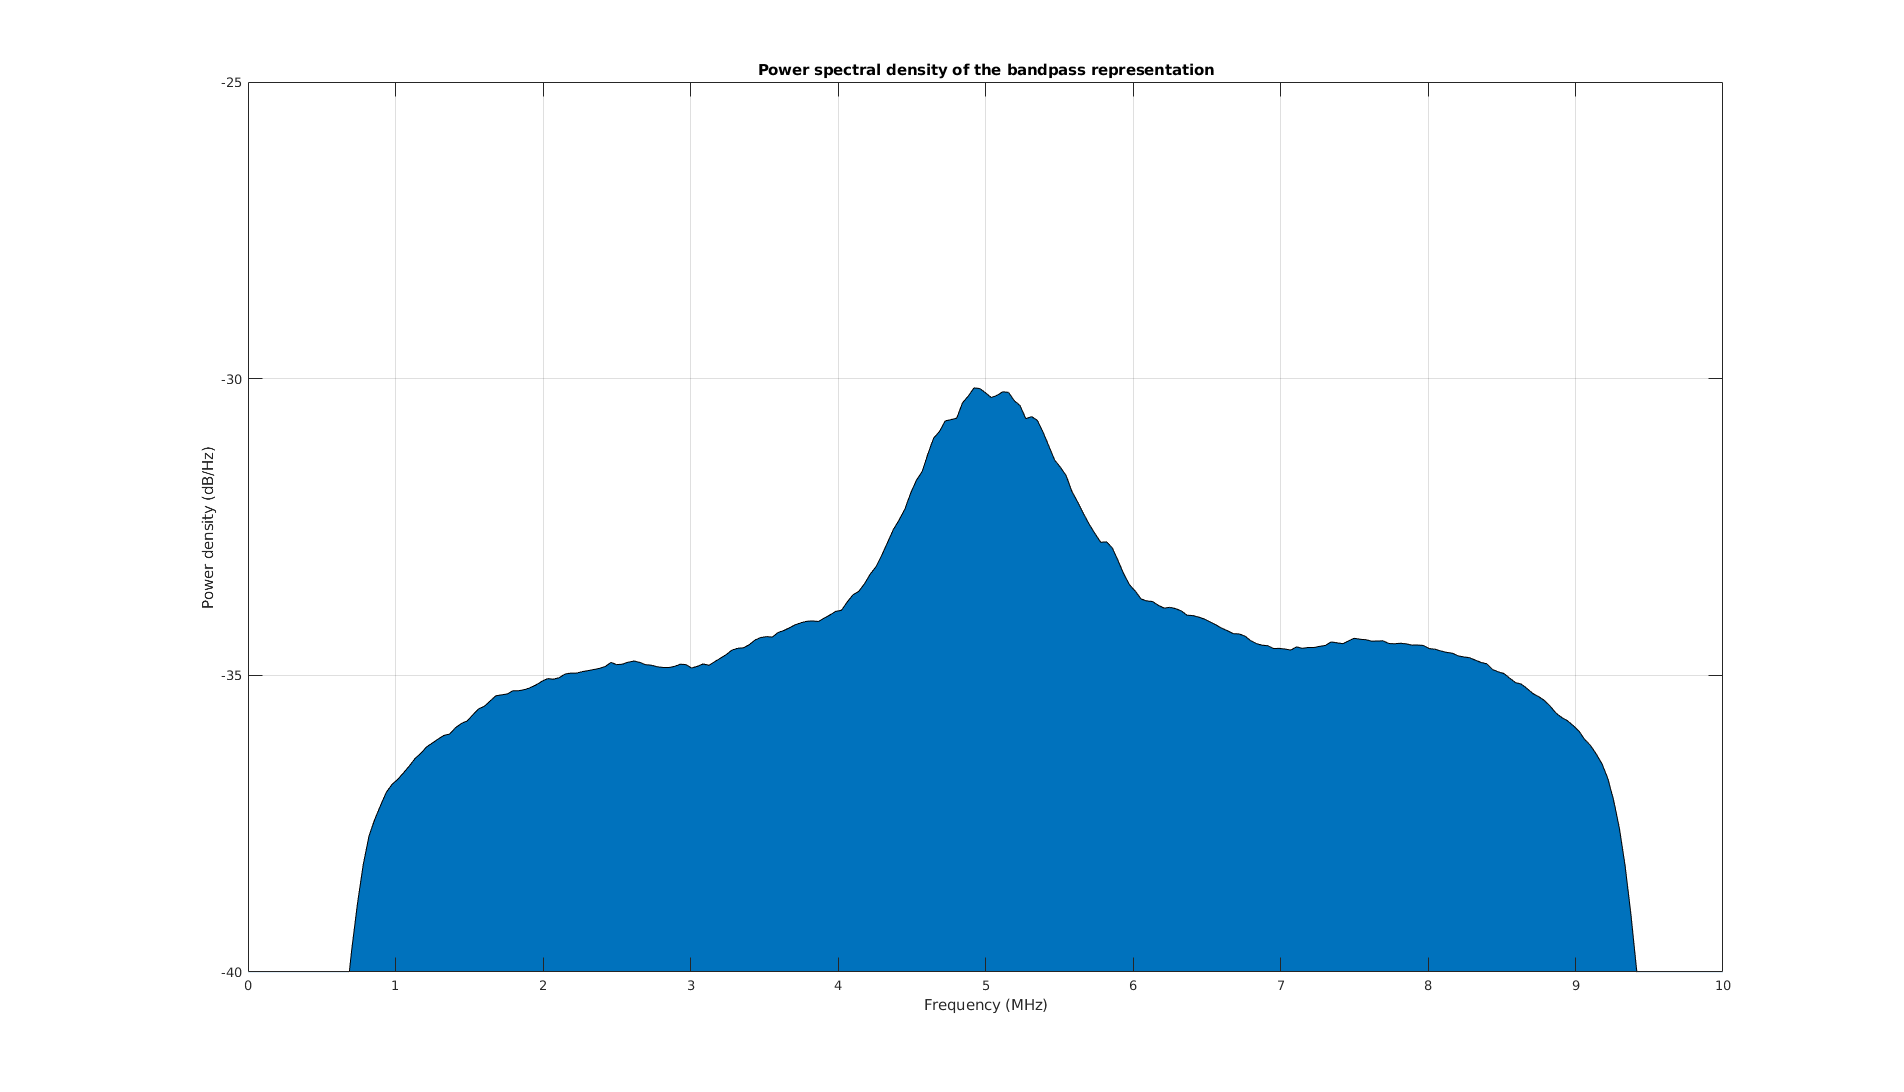
\includegraphics[width=0.9\textwidth]{figs/PSD_bandpass.png}
	\caption{Power spectral density of the bandpass representation of the original
		signal.}
	\label{fig:ex5_bandpass}
\end{figure}

\begin{figure}[H]
	\centering
	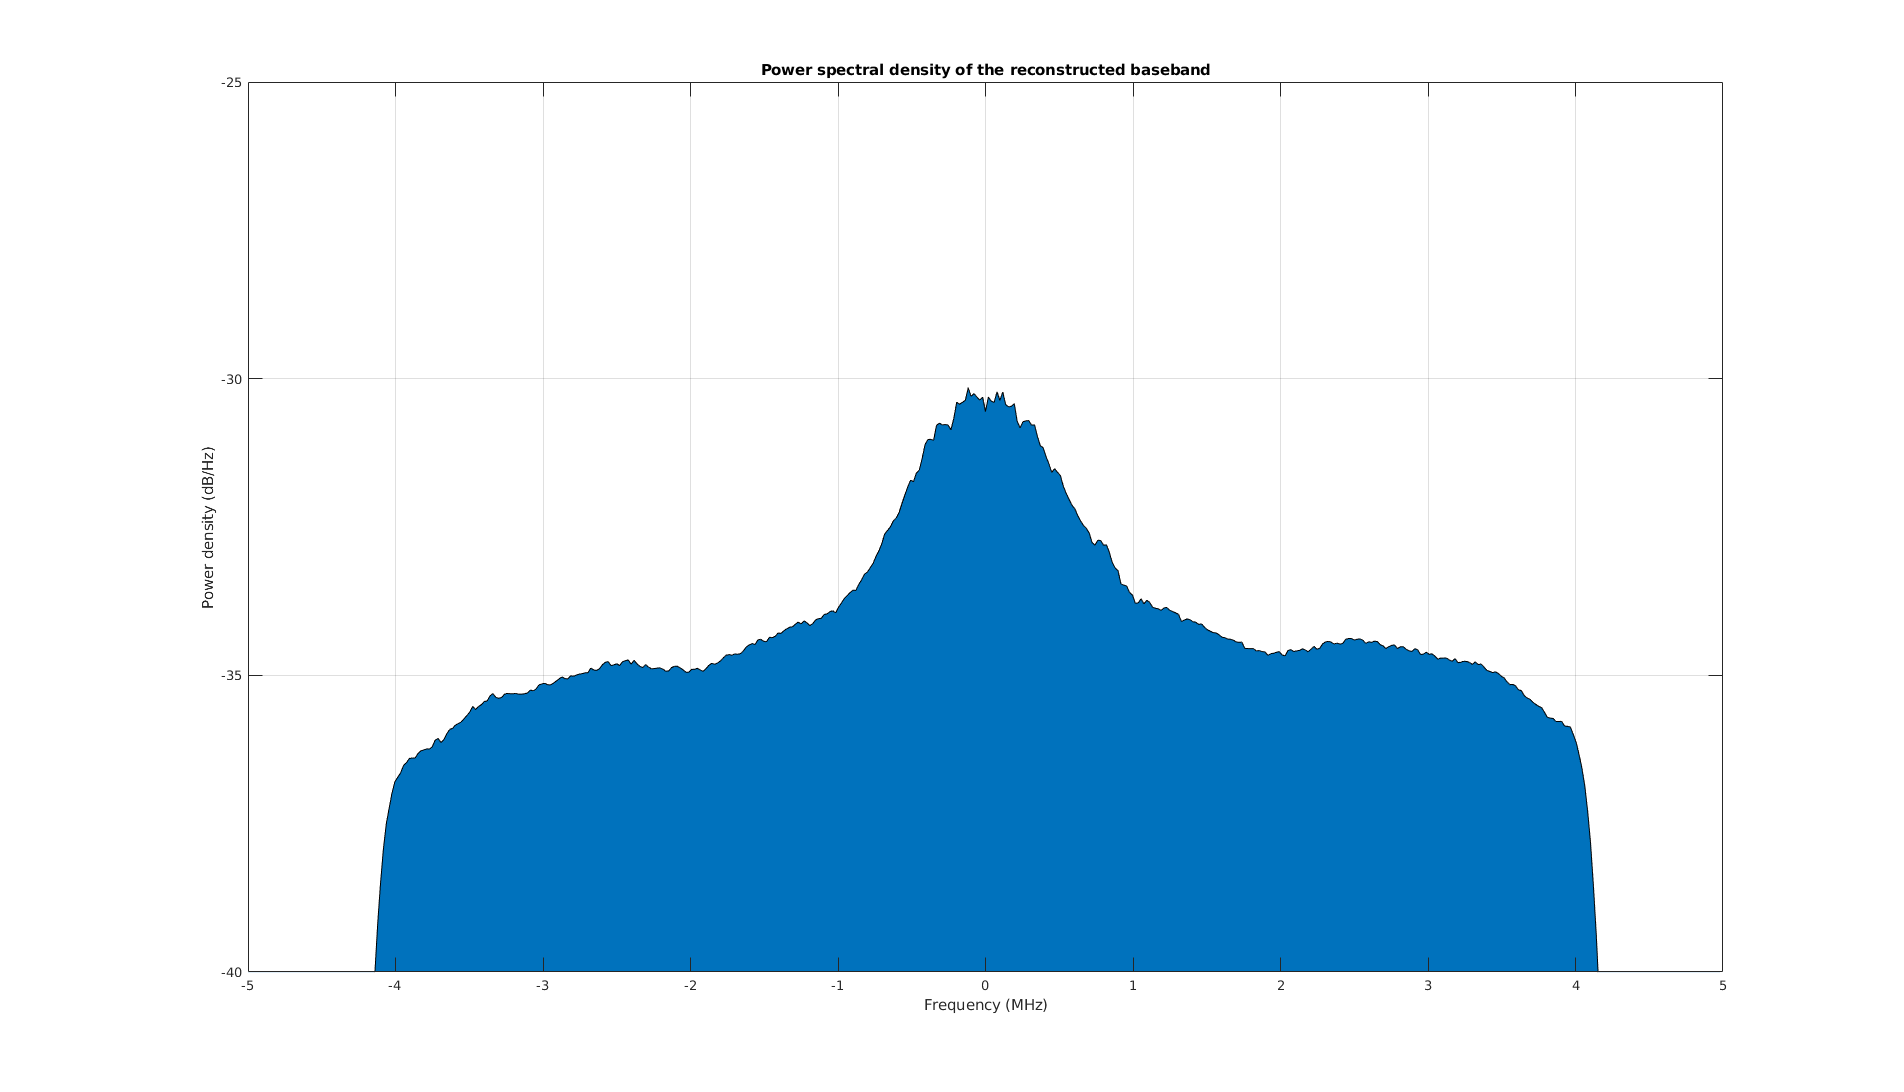
\includegraphics[width=0.9\textwidth]{figs/PSD_baseband_reconstructed.png}
	\caption{Power spectral density of the reconstructed signal in its baseband
		representation.}
	\label{fig:ex5_baseband_reconstructed}
\end{figure}

It can it seen from the graphs that the manipulation of the original signal
by processing it with the functions \textbf{iq2if} and \textbf{if2iq} slightly
changes the PSD, it makes it smoother. This is consistent with the fact that
these functions internally apply a low pass filter and therefore some of the
edges end up a little bit more rounded than originally.
